
%Copyright (C) 2016 by Krishneel@JSK Lab, The University of Tokyo

\documentclass{standalone}
\begin{document}

\subsection{Hardware}
For task 3, we used two types of UAVs; the $Hawk$ which is similar to the one used in task 1 and a transformable UAV called $snake$.
Since all the UAVs uses the same custom built control board, the center control hardware parts are almost as same as the task 1, except that we additionally designed anther PCB board for controlling the Electronic-Magnet. We equipped 5 Elec-Magnet in the UAV and build the attachment with tactile sensors. The Elec-Magnet control board is connected to the center control unit through CAN bus.

For the snake-like UAV, we program it to grasp the treasure, so the thing is different...

\subsection{Software Approach}
Just like other tasks the softwares are build on ROS environment and some functionalities are shared from task 1. Point Cloud and OpenCV libraries are used for visual perception. % target detection and motion planning are different.

\subsubsection{General Approach}
%The software system is based on ROS(Robot Operation System). We write our algorithm to the every single node and communicate with each node. 
Basically for task 3, we divide the task into three states: Search, Pick and Place. The UAVs are always within these three states and the states automatically transferred to the next one if the certain condition is satisfied as illustrated in Fig. \ref{t3}A. In "Search" state, the drone will traverse to the center of the arena and randomly generate a search end-point, the treasure detector will work when the drone is searching, once the object is detected and locked, a pick motion will be generated in the "Pick" state, the UAV will open the Elec-Magnet and moving approach to the treasure. The transfer state signal depends on the trigger of the tactile sensor, once the Elec-Magnet catch the treasure, the UAV enters "Place" state, it will directly fly to the placing zone and find the box to place the treasure. After release the treasure upon the place box, the UAV re-enter the "Search" state and loops until task is completed.

 \begin{figure}%[hb]
    \begin{center}
      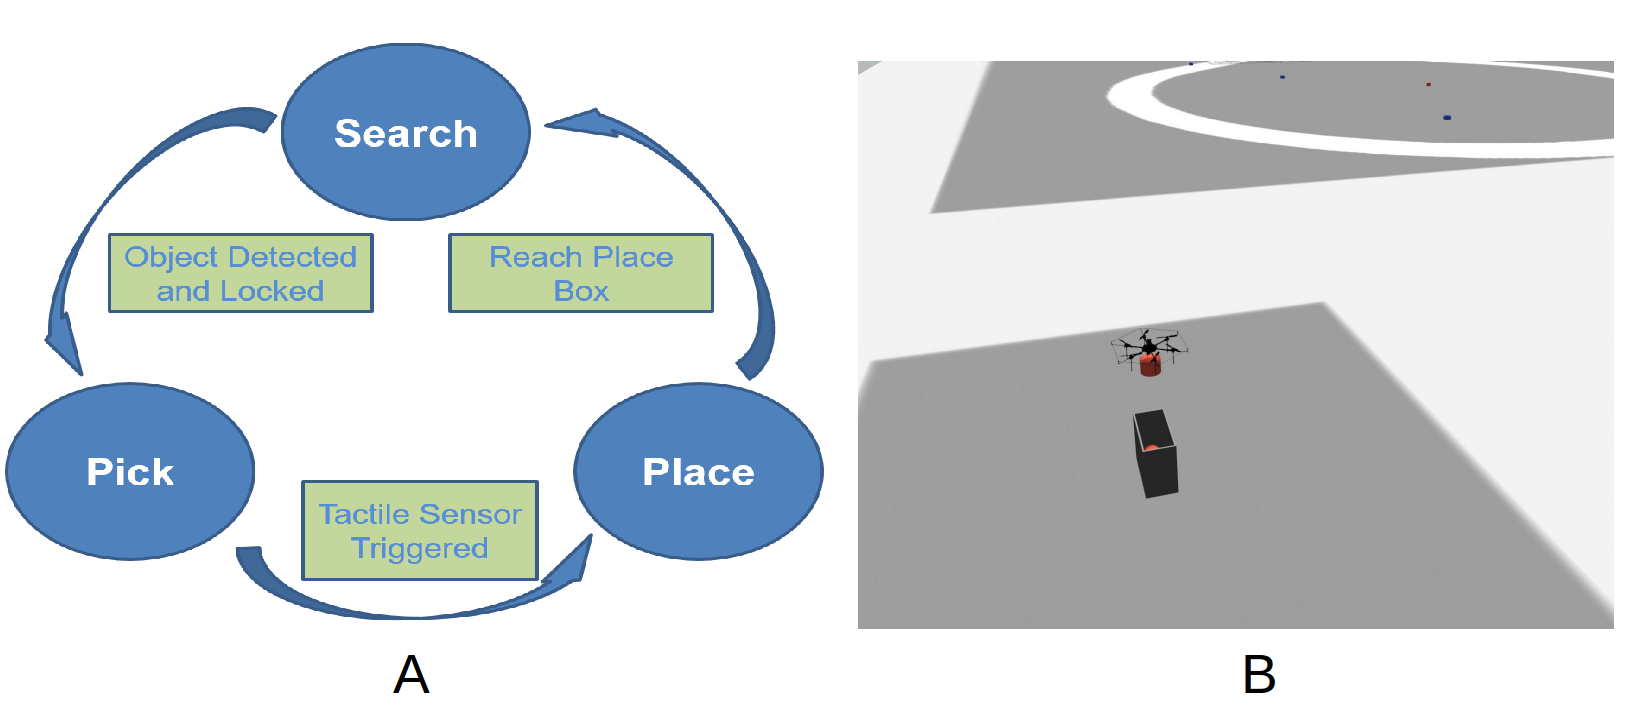
\includegraphics[keepaspectratio=true, width=1\linewidth, height=0.30\textheight]{img//task3.png}
    \end{center}
    \caption{Task 3 Demonstration}
    \label{t3}
  \end{figure}



\subsubsection{Treasure Detection}
As the treasures have distinct color features compared to the ground, we firstly used a simple detection method to localize the treasure. 
The inputs are 3D points $p_i$ from the Stereo sensor and the RGB image projection to the ground by the projection matrix computed using the known camera parameters. %We first apply 
HSI color filter is applied to obtain to 3D point candidates of treasure from the point cloud data. Next we apply Euclidean clustering to the filtered point cloud $P_{hsi}$. Euclidean clustering technique can organize points into clusters with respect to the distance feature in 3D space. For $\forall p_i, p_j \in P_{hsi}$, clusters $O_i = \{p_i \in P_i\}$ and $O_j = \{p_j \in P_j\}$ are obtained by:
\begin{equation}\label{eq3-1}
min||p_i - p_j|| \geq d_{threhold} 
\end{equation}
When we get all the clusters, we apply a simple tracker to every cluster center and as we continue to detect the same cluster over time space, the weight of the tracker is increased to boost the confidence of tracking. For clusters that are not always detected the confidence are slowly decreased and removed from the treasure candidates vector. The UAV will lock the cluster candidate when the weight is large enough and switch into the "Pick" mode to approach the treasure.

\subsection{Results Achieved to Date}
We first perform full automatic simulation in gazebo environment as shown in Fig.\ref{t3}B. To fully simulate the real scene, we add noise and outliers to the detection. In simulation, the UAV takes almost 70$seconds$ to detect, pick and place a single object. In future we will use three UAVs in coordination to complete the task which will not only decrease the time but also can be used to transport larger treasures which a single UAV might not be able to lift.
% we believe we can do that better. 
For real robot, we tested with tele-operation control, both Hawk and transformable UAV can grasp the treasure, pick and place into a specificed box. We are planing to perform more test on the real robot to justify the detection and motion planning algorithm in the simulation as part of the future work.


\end{document}
